\documentclass{oci}
\usepackage[utf8]{inputenc}
\usepackage{lipsum}
\usepackage{tikz}
\usepackage{amsmath}

% \definecolor{color1}{HTML}{D81B60}
% \definecolor{color2}{HTML}{1E88E5}
% \definecolor{color3}{HTML}{FFC107}
\definecolor{color1}{HTML}{648FFF}
\definecolor{color2}{HTML}{DC267F}
\definecolor{color3}{HTML}{FFB000}

\title{Viaje a la playa}

\begin{document}
\begin{problemDescription}
David está organizando una salida a la playa con sus amigos.
%
Su ciudad puede ser representada por una grilla de $n$ filas y $m$ columnas.
%
Para referirnos a la celda en la fila $i$-ésima y columna $j$-ésima usamos el par
$(i,j)$.
%
El viaje debe seguir un camino que parta en la esquina superior izquierda
$(1,1)$ y termine en la esquina inferior derecha $(n,m)$.
%
Para que un camino sea válido, en cada movimiento solo se puede pasar a
una celda contigua que comparta un lado.

Adicionalmente, cada celda tiene un color asociado.
%
El color de cada celda es representado por un número $C_{(i,j)}$ que va entre $1$ y $k$.
%
Para tener un viaje \emph{agradable} se tiene que cumplir una condición: dos celdas
consecutivas del camino no pueden tener el mismo color.
%
Esto significa que si en el camino se pasa de la celda $(i_1,j_1)$ a la celda $(i_2,j_2)$
entonces $C_{(i_1,j_1)} \neq C_{(i_2,j_2)}$.

David está muy confundido al ver el mapa y necesita tu ayuda.
%
Dada la descripción del mapa, tu tarea es determinar si existe un camino agradable
y, si existe, imprimir la distancia del camino agradable más corto que lleve a la
playa.

% Por ejemplo, un mapa posible con $n = 3$, $m = 3$ y $k = 3$ es:
% \begin{gather*}
% 1\ 2\ 1\\
% 3\ 3\ 2\\
% 3\ 3\ 1
% \end{gather*}
Por ejemplo, las siguientes figuras representa un posible mapa para $n=3$, $m=3$ y $k=3$:
\begin{figure}[!h]
\centering
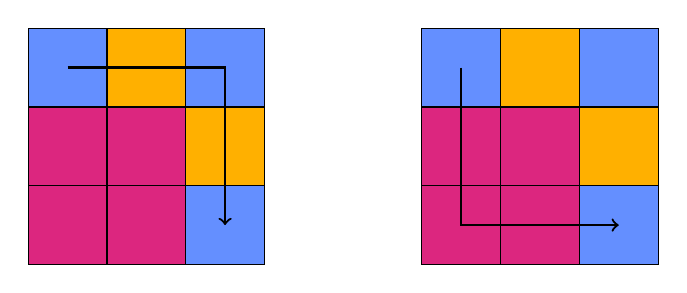
\begin{tikzpicture}
\fill[color1,draw=black] (0,0) rectangle (1,1); \fill[color3,draw=black] (1,0) rectangle (2,1); \fill[color1,draw=black] (2,0) rectangle (3,1);
\fill[color2,draw=black] (0,0) rectangle (1,-1); \fill[color2,draw=black] (1,0) rectangle (2,-1); \fill[color3,draw=black] (2,0) rectangle (3,-1);
\fill[color2,draw=black] (0,-2) rectangle (1,-1); \fill[color2,draw=black] (1,-2) rectangle (2,-1); \fill[color1,draw=black] (2,-2) rectangle (3,-1);
\draw[thick,->] (0.5,0.5) -- (2.5,0.5) -- (2.5,-1.5);

\fill[color1,draw=black] (5,0) rectangle (6,1); \fill[color3,draw=black] (6,0) rectangle (7,1); \fill[color1,draw=black] (7,0) rectangle (8,1);
\fill[color2,draw=black] (5,0) rectangle (6,-1); \fill[color2,draw=black] (6,0) rectangle (7,-1); \fill[color3,draw=black] (7,0) rectangle (8,-1);
\fill[color2,draw=black] (5,-2) rectangle (6,-1); \fill[color2,draw=black] (6,-2) rectangle (7,-1); \fill[color1,draw=black] (7,-2) rectangle (8,-1);
\draw[thick,->] (5.5,0.5) -- (5.5,-1.5) -- (7.5,-1.5);
\end{tikzpicture}
\end{figure}

Cada figura muestra un camino que va desde $(1,1)$ hasta $(3,3)$.
%
El camino de la figura de la izquierda es agradable, pero el de la derecha
no lo es, ya que la segunda, tercera y cuarta casilla son del mismo color.
%
La distancia en ambos caminos es $4$.

\end{problemDescription}


\begin{inputDescription}
La primera línea contiene tres enteros $n, m$ y $k$
($1 \leq n, m \leq 1000$, $2 \leq n\times m \leq 10^5$ y $2 \leq k \leq n \times m$)
que corresponden a las dimensiones de la ciudad y la cantidad de colores que hay.

A continuación siguen $n$ líneas, cada una con $m$ enteros que van entre $1$ y $k$.
%
El $j$-ésimo entero de la $i$-ésima línea representa a $C_{(i,j)}$, el color de la celda $(i,j)$.

\end{inputDescription}

\begin{outputDescription}
Imprime la distancia del camino agradable más corto, si este no existe imprime -1.

\end{outputDescription}

\begin{scoreDescription}
  \subtask{20}
  Se probaran varios casos en que $n = 1$, es decir, el mapa es solo una fila.
  \subtask{20}
  Se probaran varios casos en que $n = 2$ y $k = 2$, es decir, son dos filas con solo dos colores.
  \subtask{20}
  Se probaran varios casos en que $n = 2$.
  \subtask{40}
  Se probaran varios casos sin más restricciones.
\end{scoreDescription}

\begin{sampleDescription}
\sampleIO{sample-1}
\sampleIO{sample-2}
\end{sampleDescription}

\end{document}
